\subsection{Diagram komponentów}
\begin{adjustwidth}{2em}{0pt}
Diagram komponentów przedstawia podział całego systemu na mniejsze podsystemy. Komponent jest to wymienny,wykonywalny fragment systemu. Zależności między komponentami są przedstawiane w postaci interfejsów tzn. jeden komponent może korzystać z funkcji jakie udostępnia inny komponent. Na rysunku \ref{fig:diagram_komponentow} przedstawiony jest diagram komponentów projektowanego systemu

\begin{figure}[H]
    \centering
    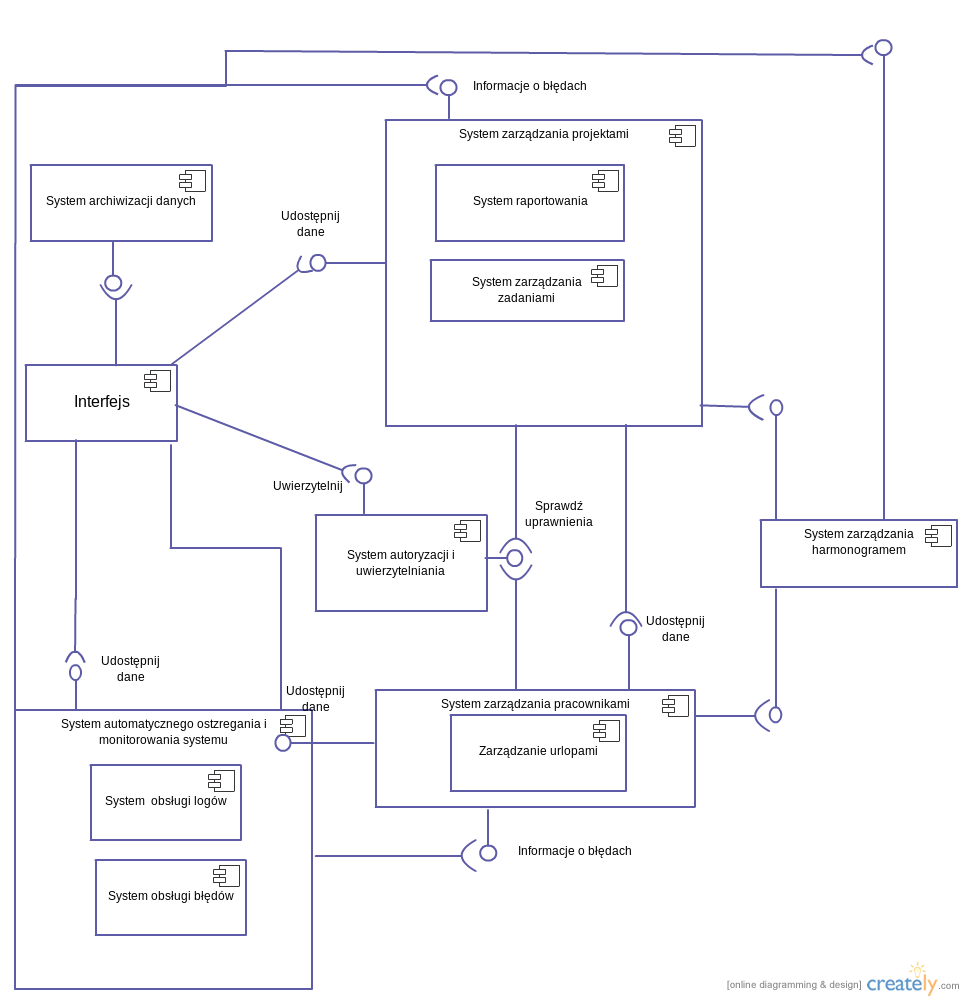
\includegraphics[scale=0.4]{diagramy/sekwencji_i_komponentow/diagram_komponentow.png}
    \caption{Diagram komponentów}
    \label{fig:diagram_komponentow}
\end{figure} 

Diagram na rysunku \ref{fig:diagram_komponentow} nie pokazuje pełnej struktury wewnętrznej wyszczególnionych podsystemów. Pokazanie zostały tylko najważniejsze komponenty tak aby rysunek pozostał czytelny. Na drugim diagramie komponentów \ref{fig:diag_kom_dane_dostep} przedstawiono w sposób bardzie szczegółowy to, że pod-systemy które korzystają z bazy danych zawierają w sobie komponenty (modele) których zadaniem jest komunikacja z bazą danych. Taka budowa systemów wynika z architektury MVC.

\begin{figure}[H]
    \centering
    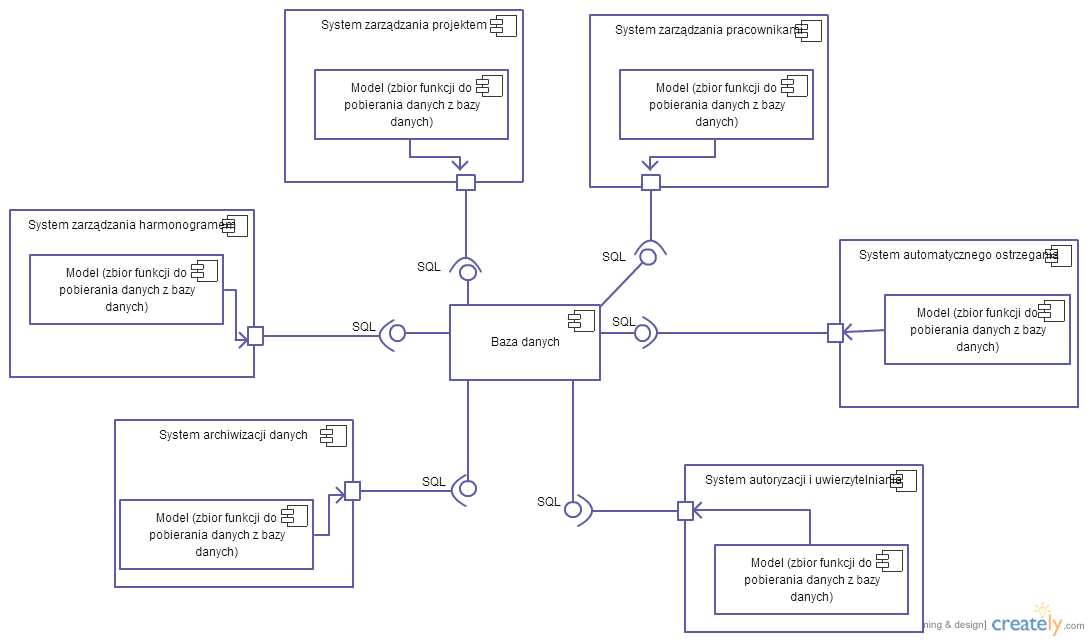
\includegraphics[scale=0.4]{diagramy/sekwencji_i_komponentow/diag_kom_dane_dostep.png}
    \caption{Diagram komponentów: dostęp do bazy danych}
    \label{fig:diag_kom_dane_dostep}
\end{figure} 

\end{adjustwidth}